% Preamble ==================================================================
\documentclass[11pt]{article}
\usepackage{geometry}
\geometry{verbose,tmargin=2.5cm,bottom= 1.5cm,lmargin=2.5cm,rmargin=2.5cm}
\usepackage{float}
\usepackage{graphicx}
\usepackage{amsmath}
\usepackage{amssymb}
\usepackage{enumitem}
\usepackage{mathtools}

\usepackage{amsthm} % theorem

\numberwithin{equation}{section}

\usepackage{titlesec,dsfont}

%Format section heading style
\usepackage{sectsty}
\sectionfont{\sffamily\bfseries\small}
\subsectionfont{\sffamily\small\slshape}
\subsubsectionfont{\sffamily\small\itshape}
\paragraphfont{\sffamily\small\textbf}


%Put period after section number
\makeatletter
\def\@seccntformat#1{\csname the#1\endcsname.\quad}
\makeatother

%Bibliography
\usepackage[round]{natbib}
\bibliographystyle{genetics}

%Format captions
\usepackage[ labelsep=period, justification=raggedright, margin=10pt,font={small},labelfont={small,normal,bf,sf}]{caption}

\setlength{\parskip}{0ex} %No space between paragraphs.

\renewcommand{\familydefault}{\sfdefault}

\newcommand\indep{\protect\mathpalette{\protect\independenT}{\perp}}
\def\independenT#1#2{\mathrel{\rlap{$#1#2$}\mkern2mu{#1#2}}}

%PUT ME LAST--------------------------------------------------
\usepackage[colorlinks=true
,urlcolor=blue
,anchorcolor=blue
,citecolor=blue
,filecolor=blue
,linkcolor=black
,menucolor=blue
,linktocpage=true
,pdfproducer=medialab
,pdfa=true
]{hyperref}

\makeatother %Put this last of all


\newcommand{\defeq}{\coloneqq}
\newcommand{\overbar}[1]{\mkern 1.5mu\overline{\mkern-1.5mu#1\mkern-1.5mu}\mkern 1.5mu}

\newtheorem{thm}{Theorem}[section]
\newtheorem{defn}{Definition}[section]
\newtheorem{cor}{Corollary}[section]

%Preamble end--------------------------------------------------


\begin{document}



\begin{flushleft}
\textbf{\Large Causal inference cheat sheet}
\end{flushleft}

\begin{flushleft}
Author: Juvid Aryaman

Last compiled: \today
\end{flushleft}

\noindent This document is a summary of useful/interesting results in causal inference, mainly from \cite{pearl09}.


\section{Basic probability}

\begin{itemize}[noitemsep]
\item Law of total probability: $P(A) = \sum_i P(A, B_i)$ (a.k.a. marginalizing over $B$)
\item Chain rule of probability: $P(A,B) = P(A|B) P(B)$
\item Thus, $P(A) = \sum_i P(A|B_i) P(B_i)$
\item Expectation: $E(g(X)) = \sum_x g(x) P(x)$
\item Conditional mean: $E(X|Y) = \sum_x x P(x|y)$
\item Variance: $\sigma_X^2 = E[(X - E(x))^2]$
\item Covariance: $\sigma_{XY} = E[(X-E(X))(Y-E(Y))]$
\item Correlation coefficient: $\rho_{XY}=\sigma_{XY}/(\sigma_X \sigma_Y)$
\item Regression coefficient of $Y$ on $X$: $r_{YX} = \rho_{XY} \sigma_Y/\sigma_X = \sigma_{XY}/(\sigma_X^2)$ (for the equation $Y = r_{YX} X + c + \mathcal{N}(0, \sigma^2)$)
\item Conditional independence: $(X \indep Y | Z) \iff P(x|y,z) = P(x|z) $
\item Partial correlation $\rho_{XY\cdot Z}$: The correlation between residuals $e_X$ and $e_Y$ resulting from the linear regression of $X$ with $Z$ and $Y$ with $Z$, respectively.
\end{itemize}


\section{Bayesian networks}
Let a \textbf{graph} $G$ consist of a set of \textbf{vertices} (or \textbf{nodes}) $V$ and a set of \textbf{edges} $E$ that connect some pair of vertices. Each edge in a graph can be either directed, undirected, or bidirected. Bidirected edges will subsequently be used to denote unobserved common causes, or \textbf{confounders}. Let a \textbf{path} be a sequence of edges such that each edge starts with the vertex ending in the preceding edge. A path may go either along or against the arrows of a directed graph. Directed graphs may include cycles (e.g.\ $X \rightarrow Y$, $Y \rightarrow X$), which represent mutual causation or feedback processes, but not self-loops (e.g. $X \rightarrow X$).

The recursive decomposition of the joint distribution into parents which characterises Bayesian networks is
\begin{equation}
P(x_1, ..., x_n) = \prod_i P(x_i|pa_i). \label{eq:bayes-net-char}
\end{equation}

\subsection{$d$-separation (blocking) in Bayesian networks} \label{sec:blocking}

Let an arrow $pa_j \rightarrow x_j$ denote part of a directed acyclic graph (DAG) in which variables are represented by nodes, and arrows are drawn from each node of the parent set $PA_j$ towards the child node $X_j$.

\begin{defn}
\textbf{$d$-separation} A path $p$ is $d$-separated (or blocked) by a set of nodes $Z$ if and only if
\begin{enumerate}[noitemsep]
\item $p$ contains a chain $i \rightarrow m \rightarrow j$ or a fork $i \leftarrow m \rightarrow j$ such that the middle node $m$ is in $Z$, or
\item $p$ contains a collider $i \rightarrow m \leftarrow j$ such that the middle node $m$ is not in $Z$ and such that no descendant of $m$ is in $Z$
\end{enumerate}
A set $Z$ d-separates $X$ from $Y$ if and only if $Z$ blocks \textbf{every} path from a node in $X$ to a node in $Y$
\end{defn}

\begin{thm}
\textbf{Probabilistic implications of $d$-separation} Consequently, if $X$ and $Y$ are $d$-separated by $Z$ in a DAG $G$, then $(X \indep Y | Z)$ in every distribution compatible with $G$. Conversely, if $X$, $Y$, and $Z$ are \textit{not} $d$-separated by $Z$ in a DAG $G$ then $X$ and $Y$ are dependent conditional on $Z$ in almost all distributions compatible with $G$ (assuming no parameter fine-tuning).
\end{thm}

\section{Functional causal models}
A functional causal model consists of a set of equations of the form
\begin{equation}
x_i = f_i(pa_i, u_i), \quad i=1,...,n \label{eq:func-caus-mod}
\end{equation}
where $pa_i$ are the set of variables (parents) that directly determine the value of $X_i$ (i.e.\ its direct causes) and $U_i$ represents errors (or ``disturbances'') due to omitted factors. Eq.\eqref{eq:func-caus-mod} is called a causal model if each equation represents the process by which the \textit{value} (not merely the probability) of variable $X_i$ is selected.

When some disturbances $U_i$ are judged to be dependent, it is customary to denote such dependencies in a causal graph with double-headed arrows. If the causal diagram is acyclic, then the corresponding model is called \textit{semi-Markovian} and the values of the variables $X$ are uniquely determined by those of the variables $U$. If the error terms $U$ are jointly independent, the model is called \textit{Markovian}.

Linear structural equation models obey
\begin{equation}
x_i = \sum_{k \neq i} \alpha_{ik} x_k + u_i, \quad i=1,...,n 
\end{equation}
In linear models, $pa_i$ corresponds to variables on the r.h.s.\ of the above equation where $\alpha_{ik} \neq 0$.

\subsection{Counterfactuals in functional causal models: An example}
Consider a randomized clinical trial, where patients are/are not treated $X \in \{0,1\}$. We also observe whether the patients die after treatment $Y\{0,1\}$. We wish to ask the question: did the patient die \textit{because of} the treatment, \textit{despite} the treatment, or \textit{regardless} of the treatment.

Assume $P(y|x) = 0.5$, and therefore $P(y,x)=0.25$ for all $x$ and $y$. We can write two models with the same joint distribution

\textit{Model 1 (treatment no effect):}
\begin{align}
&x=u_1\\
&y=u_2\\
&P(u_1=1) = P(u_2=1)= \frac{1}{2}
\end{align}


\textit{Model 2 (treatment has an effect):}
\begin{align}
&x=u_1\\
&y=xu_2 + (1-x)(1-u_2)\\
&P(u_1=1) = P(u_2=1)= \frac{1}{2}
\end{align}

Let $Q$=fraction of deceased subjects from the treatment group who would not have died had they not taken the treatment. In model 1, $Q=0$ since $X$ has no effect on $Y$. In model 2, subjects who died ($y=1$) and were treated ($x=1$) must correspond to $u_2=1$. If $u_2=1$ then the only way for $y=0$ is for $x=0$. I.e. if you are a patient for whom $u_2=1$ then the only way not to die is to not take the treatment, so the treatment caused your death. So $Q=1$.

Consequence 0: joint probability distributions are insufficient for counterfactual computation

Consequence 1: stochastic causal models are insufficient for counterfactual computation

Consequence 2: functional causal models are sufficient to define and compute counterfactual statements.

\subsection{General method to compute counterfactuals}
Given evidence $e=\{X_{obs}, Y_{obs}\}$, to compute probability of $Y=y$ under hypothetical condition $X=x$ apply the following steps:
\begin{enumerate}[noitemsep]
\item Abduction: Update the probability of disturbances $P(u)$ to obtain $P(u|e)$
\item Action: Replace the equations corresponding to variables in the set $X$ by the equations $X=x$
\item Prediction: Use the modified model to compute the probability $Y=y$.
\end{enumerate}

\section{Causal Bayesian networks}
Given two disjoint sets of variables $X$ and $Y$, the \textbf{causal effect} of $X$ on $Y$, denoted as $P(y|\hat{x})$ or $P(y|do(x))$, is the probability of $Y=y$ by deleting all equations from Eq.\eqref{eq:func-caus-mod} where variables $X$ are on the l.h.s., and substituting $X=x$ in the remaining equations.

This corresponds to mutilating the DAG such that all arrows pointing directly to $X_i$ are removed. \textbf{Amputation is the difference between seeing and doing}.

For an atomic intervention, we get the \textit{truncated factorization} formula
\begin{equation}
P(x_1,...,x_n|\hat{x}'_i)=\begin{dcases}
\prod_{j\neq i} P(x_j|pa_j) \quad &\text{if}\ x_i = x_i'\\
0 &\text{if}\ x_i \neq x_i'
\end{dcases}
\end{equation}
The $j\neq i$ denotes the removal of the term $P(x_i|pa_i)$ from Eq.\eqref{eq:bayes-net-char} (i.e. amputation). A $do(x_i)$ is a severely limited sub-space of the full joint distribution, since the distribution only has support where the intervention variable $x_i$ is equal to its particular intervention value $x_i'$, rather than a continuum of values in Eq.\eqref{eq:bayes-net-char}.

Multiplying and dividing by $P(x'_i|pa_i)$ yields
\begin{equation}
P(x_1,...,x_n|\hat{x}'_i)=\begin{dcases}
P(x_1,...,x_n|x_i',pa_i)P(pa_i) \quad &\text{if}\ x_i = x_i'\\
0 &\text{if}\ x_i \neq x_i'
\end{dcases}
\end{equation}
Marginalization of the above leads to the following theorem.

\paragraph{Adjustment for direct causes} 
Let $PA_i$ denote the set of direct causes of variable $X_i$, and let $Y$ be any set of variables disjoint of $\{X_i \cup PA_i \}$. The causal effect of $do(X_i=x_i')$ on $Y$ is
\begin{equation}
P(y|\hat{x}_i') = \sum_{pa_i} P(y | x'_i, pa_i) P(pa_i)
\end{equation}
where $P(y|x_i', pa_i)$ and $P(pa_i)$ are preintervention probabilities. This is called ``adjusting for $PA_i$''.


\paragraph{Identifiability}
Causal quantities are defined relative to a causal model $M$, not the joint distribution $P_M(v)$ over the set of observed variables $V$. Non-experimental data provides information about $P_M(v)$ alone, and several graphs can give rise to the same $P_M(v)$. Thus, not all quantities are unambiguously \textbf{identifiable} from observational data, \textbf{even with infinite samples}. Added assumptions by specifying a particular $M$ can provide enough details to compute quantities of interest without explicating $M$ in full.

Theorem 3.2.5: Given a causal diagram $G$ of any Markovian model in which a subset of variables $V$ are measured, the causal effect $P(y|\hat{x})$ is identifiable whenever $\{X \cup Y \cup PA_X\} \subseteq V$. I.e. \textit{all parents of the cause are necessary to estimate the causal effect}.

\section{Inferring causal structure}
\begin{itemize}
\item IC algorithm is for inferring causal structure given observational data when there are no latent variables
\item IC* algorithm is for inferring causal structure given observational data when there are latent variables. The PC algorithm is apparently more contemporary (see \cite{spirtes10})
\item There are local criteria for potential cause and genuine cause
\item Spurious association: $X$ and $Y$ are spuriously associated if they are dependent in some context and there exists a latent common cause, as exemplified in the structure $Z_1 \rightarrow X \rightarrow Y \leftarrow Z_2$
\item NOTEARS \citep{zheng18} casts the structure learning problem as a continuous optimization problem over real matrices to avoid the superexponential combinatorial explosion with number of variables.
\end{itemize}

\section{Adjusting for confounding bias}

When seeking to evaluate the effect of one factor ($X$) on another ($Y$), we should ask \textbf{whether} we should \textit{adjust} for possible variations in other factors ($Z$, known as ``covariates'', ``concomitants'' or ``confounders''). This becomes apparent in \textbf{Simpson's paradox}: any statistical relationship between two variables may be reversed by including additional factors in the analysis.

\subsection{The back-door criterion}
This criterion demonstrates how confounders that \textit{affect} the treatment variable can be used to facilitate causal inference.

\begin{figure}
\begin{center}
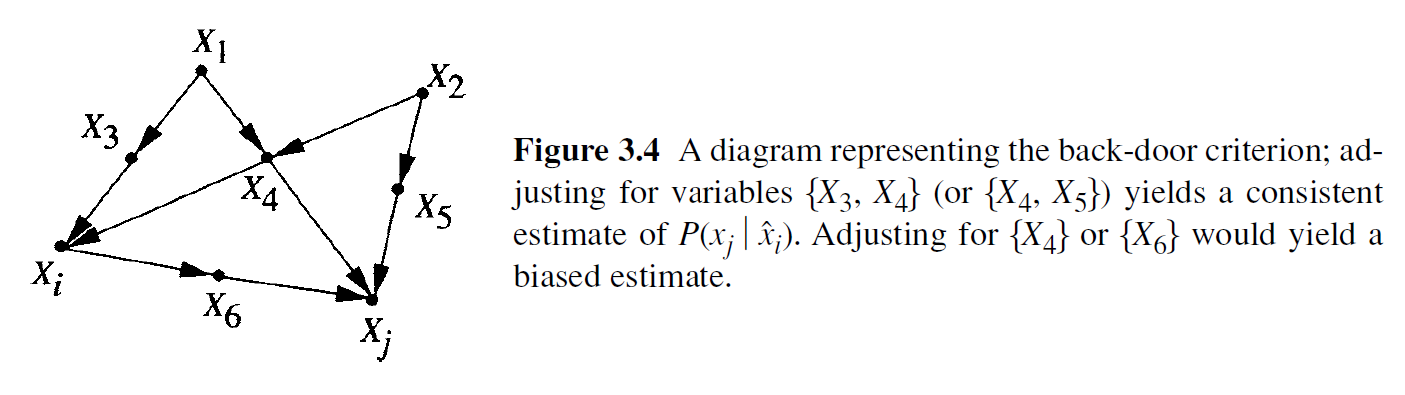
\includegraphics[width=0.8\columnwidth]{figures/back-door.png}  
\end{center}
\caption{Example of the back-door criterion
}
\label{Fig:front_door}
\end{figure}

\paragraph{Back-door} 
A set of variables $Z$ satisfy the back-door criterion relative to an ordered pair of variables ($X_i$,$X_j$) in a DAG $G$ if:
\begin{enumerate}[noitemsep]
\item no node in $Z$ is a descendant of $X_i$; and
\item $Z$ blocks every path between $X_i$ and $X_j$ that contains an arrow into $X_i$
\end{enumerate}
Similarly, if $X$ and $Y$ are two disjoint subsets of nodes in $G$, then $Z$ satisfies the back-door criterion relative to $(X,Y)$ if it satisfies the criterion relative to any pair $(X_i, X_j)$ such that $X_i \in X$ and $X_j \in Y$.

\paragraph{Back-door adjustment}
If a set of variables $Z$ satisfies the back-door criterion relative to $(X,Y)$, then the causal effect of $X$ on $Y$ is identifiable and is given by
\begin{equation}
P(y|\hat{x}) = \sum_z P(y|x,z)P(z).
\end{equation}
This corresponds to partitioning the population into groups that are homogeneous relative to Z, assessing the effect of X on Y in each homogeneous group, and then averaging the results. Conditioning in this way means that the observation $X=x$ cannot be distinguished from an intervention $do(x)$.

\subsection{The front-door criterion}
This criterion demonstrates how confounders that are \textit{affected by} the treatment variable can be used to facilitate causal inference.

\begin{figure}
\begin{center}
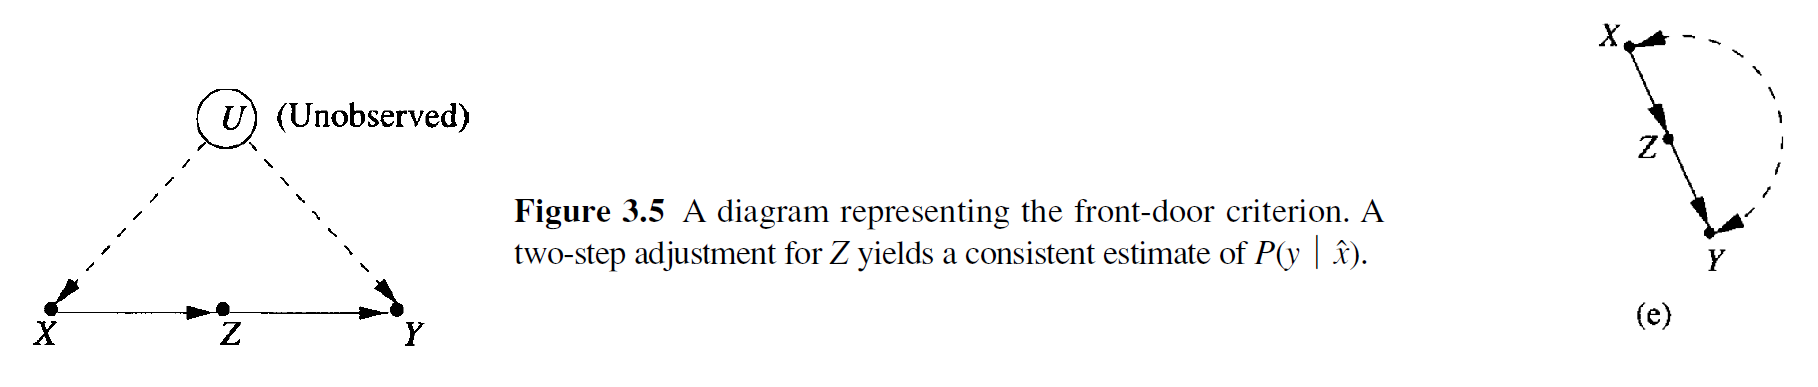
\includegraphics[width=0.8\columnwidth]{figures/front-door.png}  
\end{center}
\caption{(Left) Example of the front-door criterion. The path $X \leftarrow U \rightarrow Y$ denotes an unobserved (latent) unobserved common cause. (Right) This is often represented as a \textbf{bi-directed path}. 
}
\label{Fig:front_door}
\end{figure}

\paragraph{Front-door} 
A set of variables $Z$ satisfy the front-door criterion relative to an ordered pair of variables $(X, Y)$ if:
\begin{enumerate}[noitemsep]
\item $Z$ intercepts all directed paths from $X$ to $Y$; 
\item there is no unblocked back-door path from $X$ to $Z$; and
\item all back-door paths from $Z$ to $Y$ are blocked by $X$.
\end{enumerate}

\paragraph{Front-door adjustment}
If $Z$ satisfies the front-door criterion relative to $(X, Y)$ and if $P(x, z) > 0$, then the causal effect of $X$ on $Y$ is identifiable and is given by
\begin{equation}
P(y|\hat{x}) = \sum_z P(z|x) \sum_{x'} P(y|x',z)P(x')
\end{equation}

Conditions (2) and (3) of the front-door definition are overly restrictive: e.g. nested combinations of back-door and front-door conditions are permissible (see Section~\ref{sec:do-calc} for a more general set of conditions).

\section{Do-calculus} \label{sec:do-calc}

The back-door and front-door criteria do not provide a complete set of rules for when/how causal effects can be computed. Do-calculus sidesteps the need for algebraic manipulation and provides a complete set of inference rules by which probabilistic sentences involving interventions and observations can be transformed into other such sentences, allowing a method of deriving/verifying claims about interventions. The aim is to compute causal effect expressions for $P(y|\hat{x})$ where $Y$ and $X$ are subsets of variables. When $P(y|\hat{x})$ can be reduced to an expression involving observable probabilistic quantities, we say that the causal effect of $X$ on $Y$ is \textbf{identifiable}.

\subsection{Notation}
\begin{itemize}[noitemsep]
\item $G_{\overline{X}}$ = graph obtained by deleting from $G$ all arrows pointing into nodes in $X$
\item $G_{\underline{X}}$ = graph obtained by deleting from $G$ all arrows pointing out of nodes in $X$
\item $G_{\overline{X}\underline{Z}}$ = graph obtained by deleting from $G$ all arrows pointing into nodes in $X$ and out of nodes in $Z$
\item $P(y|\hat{x},z) \defeq P(y,z|\hat{x}) / P(z|\hat{x})$, meaning the probability of observing $Y=y$ given an \textit{intervention} $X=x$ and an \textit{observation} $Z=z$
\end{itemize}

\subsection{Rules} \label{sec:Rules}

\paragraph{Rule 1} (Insertion/deletion of observations)
\begin{equation}
P(y|\hat{x}, z, w) = P(y| \hat{x}, w) \quad \text{if}\ (Y \indep Z|X,W)_{G_{{\overline{X}}}}.
\end{equation}

This rule is a reaffirmation of $d$-separation (Section~\ref{sec:blocking}) as a valid test for conditional independence in the distribution resulting from $do(X=x)$. The rule follows from the fact that deleting equations from the system ($G_{{\overline{X}}}$) does not introduce any dependencies among the remaining disturbance terms.


\paragraph{Rule 2} (Action/observation exchange)
\begin{equation}
P(y|\hat{x},\hat{z},w) = P(y|\hat{x},z,w) \quad \text{if}\ (Y \indep Z|X,W)_{G_{{\overline{X}\underline{Z}}}}.
\end{equation}

This rule provides a condition for an external intervention $do(Z=z)$ to have the same effect on $Y$ as the passive observation $Z=z$. The condition amounts to $\{X \cup W\}$ blocking all back-door paths from $Z$ to $Y$ (in $G_{\overline{X}}$), since $G_{\overline{X}\underline{Z}}$ retains all (and only) such paths.

\paragraph{Rule 3} (Insertion/deletion of actions)
\begin{equation}
P(y|\hat{x},\hat{z},w) = P(y|\hat{x},w) \quad \text{if}\ (Y \indep Z|X,W)_{G_{{\overline{X},\overline{Z(W)}}}}
\end{equation}
where $Z(W)$ is the set of $Z$-nodes that are not ancestors of any $W$-node in $G_{\overline{X}}$.

This rule provides conditions for introducing (or deleting) an external intervention $do(Z=z)$ without affecting the probability of $Y=y$. The validity of this rule stems from simulating the intervention $do(Z=z)$ by the deletion of all equations corresponding to the variables in $Z$ (hence $G_{\overline{X} \overline{Z}}$).

\paragraph{Completeness} A quantity $Q=P(y|do(x),z)$ is identifiable if and only if it can be reduced to a \textit{do}-free expression using the above 3 rules.

\subsection{Identifiability}
A causal effect $q = P(y_1, \dots, y_k| \hat{x}_1, \dots, \hat{x}_m)$ is identifiable in a model characterised by a graph $G$ is there exists a finite sequence of transformations conforming to one of the three rules in Section~\ref{sec:Rules} that reduces $q$ into a standard (i.e.\ ``hat''-free) probability expression involving observed quantities. Figure \ref{Fig:graph_cond_ci} provides a set of graphical conditions; if any one is satisfied then $P(y|\hat{x})$ is identifiable, and satisfying at least one of the conditions is necessary for $P(y|\hat{x})$ to be identifiable. I.e. $P(y|\hat{x})$ is unidentifiable then no finite sequence of inference rules reduces $P(y|\hat{x})$ to a hat-free expression. Figure \ref{Fig:graph_cond_ci} can also be used to define an algorithm for deriving a closed-form expression for control queries in terms of observable quantities, an implementation in \texttt{R} is in the package \texttt{causaleffect}, see \cite{tikka17} and a Jupyter Notebook example \href{https://github.com/jaryaman/ML_demos/blob/master/Notebooks/do-calculus.ipynb}{here}.


\begin{figure}
\begin{center}
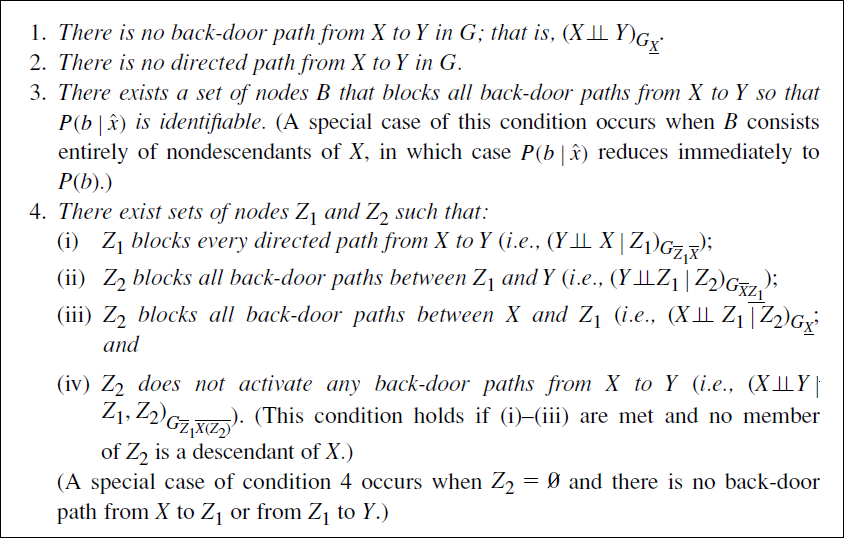
\includegraphics[width=0.8\columnwidth]{figures/graph-cond-ident-4-3-1.png}  
\end{center}
\caption{Graphical conditions for identification of causal effect (Theorem 4.3.1 Causality). Satisfying at least one renders the causal effect $P(y|\hat{x})$ identifiable, whereas satisfying none implies unidentifiability of the causal effect.}
\label{Fig:graph_cond_ci}
\end{figure}

\paragraph{Assorted facts on identifiability} 

\begin{itemize}
\item Whilst a causal effect is not identifiable for \textit{every} joint distribution of variables if this condition is broken, it might be for \textit{some} probability densities. For example, an instrumental variable can yield a causal effect identifiable in a linear model in the the presence of a bow pattern (Fig.~3.7A of Causality), but will not be generally identifiable (see Section 3.5 of Causality).
\item If $P(y|\hat{x})$ is identifiable, then if a set of nodes $Z$ lies on a directed path from $X$ to $Y$, then $P(z|\hat{x})$ is also identifiable (lemma 4.3.4).
\item \textbf{Complete identifiability condition} A sufficient condition for identifying the causal effect $P(y|do(x))$ is that there exists no bi-directed path (i.e.\ a path composed entirely of bi-directed arcs, see Fig.~\ref{Fig:front_door}) between $X$ and any of its children. Prior to applying this criterion, all nodes which are not ancestors of $Y$ are deleted from the graph (i.e.\ only consider nodes which are on pathways from $X$ to $Y$).
\end{itemize}

\section{Actions, plans, and direct effects}

Pearl defines two kinds of intervention:

\begin{itemize}[noitemsep]
\item Act: An intervention which results from a reactive policy, deriving from an agent's beliefs, disposition, and environmental inputs (or the ``outside'')
\item Action: An intervention which results from a deliberative policy, deriving from an agent's free will (or the ``inside''; meditative traditions might not draw such a bright line between these two classifications as a  description of physical reality, but it is no doubt a useful distinction for reasoning about the future when conscious agents are involved)
\end{itemize} 

\subsection{Conditional actions and stochastic policies}
In general, interventions may involve complex policies in which $X$ is made to respond according to e.g. a deterministic functional relationship $x=g(z)$, or more generally through a stochastic relationship whereby $X$ is set to $x$ with probability $P^*(x|z)$. 


Let $P(y|do(X=g(z)))$ denote the distribution of $Y$ prevailing under the deterministic policy $do(x=g(z))$. Then,
\begin{align}
P(y|do(X=g(z))) &= \sum_z P(y|do(X=g(z)),z) P(z|do(X=g(z))) \\
&= \sum_z P(y|\hat{x}, z)|_{x=g(z)} P(z) \nonumber \\
&= E_z[P(y|\hat{x},z)|_{x=g(z)}]. \nonumber
\end{align}
Hence, the evaluation of the outcome of an intervention under a complicated conditional policy $x=g(z)$ amounts to being able to evaluate $P(y|\hat{x},z)$. The equality $P(z|do(X=g(z))) = P(z)$ stems from the fact that $Z$ \textbf{cannot} be a descendant of $X$: in other words, \textbf{one cannot define a coherent policy of action for $X$ based on an (indirect) effect of $X$ because actions change the distributions of their effects!} (Aside: I suppose one might argue about whether an agent has any choice over the form of $g(z)$)

Similarly, let $P(y)|_{P^*(x|z)}$ denote the distribution of $Y$ prevailing under the stochastic policy $P^*(x|z)$ -- i.e.\ given $Z=z$, $do(X=x)$  occurs with probability $P^*(x|z)$. Then,
\begin{equation}
P(y)|_{P^*(x|z)} = \sum_x \sum_z P(y|\hat{x}, z) P^*(x|z) P(z).
\end{equation}
Since $P^*(x|z)$ is specified externally, it is again the case that $P(y|\hat{x}, z)$ is sufficient for the identifiability of any stochastic policy which shapes the distribution of $X$ by the outcome of $Z$.


\subsection{Identification of dynamic plans}

A \textbf{control problem}  consists of a DAG with vertex set $V$ partitioned into four disjoint sets $V=\{X,Z,U,Y\}$ where
\begin{itemize}
\item $X=$ the set of control variables (exposures, interventions, treatments, etc.)
\item $Z=$ the set of observed variables, often called \textbf{covariates}
\item $U=$ the set of unobserved (latent) variables, and
\item $Y=$ an outcome variable
\end{itemize}
We are interested in settings where we have gathered data $\mathcal{D}=\{X,Z,Y\}$ for previous agents making actions $X$. The problem is, given a new instance of the system (e.g.\ a new patient whom we seek to treat), can we estimate the outcome of $\{do(x_1),...,do(x_n)\}$ using only the observational data $\mathcal{D}$. See Section 4.4.1 of Causality for a specific motivating example.

Let control variables be ordered $X=X_1,...,X_n$ such that every $X_k$ is a non-descendant of $X_{k+j}$ ($j>0$) and let the outcome $Y$ be a descendant of $X_n$. A \textbf{plan} is an ordered sequence $(\hat{x}_1,...,\hat{x}_n)$ of value assignments to the control variables. A \textbf{conditional plan} is an ordered sequence $(\hat{g}_1(z_1),...,\hat{g}_n(z_n))$ where $\hat{g}_k(z_k)$ means ``set $X_k$ to $\hat{g}_k(z_k)$ whenever $Z_k=z_k$'', where the support $Z_k$ of each $g_k(z_k)$ must not contain any variables that descendants of $X_k$.

\begin{thm}
\textbf{Plan identification: the sequential back-door criterion}. The probability of the \textbf{unconditional} plan $P(y|\hat{x_1}, ..., \hat{x}_n)$ is identifiable if, for every $1 \leq k \leq n$ there exists a set $Z_k$ of covariates satisfying the following conditions:
\begin{equation}
Z_k \subseteq N_k
\end{equation}
where $N_k$ is the set of observed nodes that are non-descendants of any element of $\{X_k, X_{k+1},...,X_n\}$, and
\begin{align}
(Y \indep X_k | X_1,...,X_{k-1},Z_1,...,Z_k)_{{G_{\underline{X}_k,\overline{X}_{k+1},...,\overline{X}_{n}}}}
\end{align}
When these conditions are satisfied, the effect of the plan is given by
\begin{align}
P(y|\hat{x}_1,...,\hat{x}_n) = \sum_{z_1,...,z_n} P(y|z_1,...,z_n,x_1,...,x_n) \times \prod_{k=1}^n P(z_k|z_1,...,z_{k-1},x_1,...,x_{k-1})
\end{align}
\end{thm}

\subsection{Direct and indirect effects}

We are often concerned with the extent to which a variable affects another directly, rather than the total causal effect mediated through all other intervening variables. For example, in cases of sex discrimination, we may be interested in asking the direct effect of an applicant's sex on the outcome of an applicant's job application. In effect, we are concerned with the causal effect of variable $X$ on $Y$ while all other factors in the analysis are held fixed (\textit{Ceteris paribus}).

\begin{defn}
\textbf{Direct effect}. The direct effect of $X$ on $Y$ is given by $P(y|\hat{x},\hat{s}_{XY})$ where $\hat{s}_{XY}$ is the set of all endogenous variables (i.e.\ variables in the model) except $X$ and $Y$
\end{defn}

\begin{cor}
The direct effect of $X$ on $Y$ is given by $P(y|\hat{x}, \hat{pa}_{Y \setminus X})$ where $pa_{Y \setminus X}$ is any realization of the parents of $Y$ excluding $X$.
\end{cor}

It is sometimes meaningful to average the direct effect over all levels of $pa_{Y\setminus X}$. To do this, we define the natural direct effect:

\begin{defn}
\textbf{Natural direct effect}. The natural direct effect ($DE_{x,x'}(Y)$) is defined as
\begin{equation}
DE_{x,x'}(Y) = E[Y(x', Z(x)) - E(Y(x))]
\end{equation}
where $Z= pa_{Y\setminus X}$, and $Y(x', Z(x))$ is the value that $Y$ would attain under the counterfactual scenario of $X=x'$, but $Z$ retaining the values under the setting $X=x$.
\end{defn}

The natural direct effect involves probabilities of nested counterfactuals, and cannot generally be written in terms of the $do(x)$ operator. However, if certain assumptions of ``no confounding'' are deemed valid, the natural direct effect can be reduced to 

\begin{equation}
DE_{x,x'}(Y) = \sum_z [E(Y|do(x', z)) - E(Y| do(x,z))]P(z|do(x))
\end{equation}
which is simply a weighted average of controlled direct effects. 

We can also define the indirect effect which quantifies the influence of $X$ on $Y$ through all paths except for the direct path from $X \rightarrow Y$.
\begin{defn}
\textbf{Indirect effect}. The natural indirect effect ($IE_{x,x'}(Y)$) is defined as
\begin{equation}
IE_{x,x'}(Y) = E[Y(x, Z(x')) - E(Y(x))]
\end{equation}
\end{defn}
We can define the total effect of a transition to be the \textit{difference} between the direct effect of that transition and the indirect effect of the reverse transition
\begin{defn}
\textbf{Total effect}. The total effect ($TE_{x,x'}(Y)$) is defined as
\begin{equation}
TE_{x,x'}(Y) \defeq E[Y(x') - E(Y(x))] = DE_{x,x'}(Y) - IE_{x',x}(Y)
\end{equation}
\end{defn}

\section{Causality and structural models}

Let's rewrite Eq.\eqref{eq:func-caus-mod} as
\begin{equation}
x_i = f_i(pa_i, \epsilon_i), \quad i=1,...,n. 
\end{equation}


In general, for the \textbf{partial correlation} $\rho_{XY\cdot Z}$, 
\begin{equation}
(X \indep Y | Z) \implies \rho_{XY\cdot Z} = 0 
\end{equation}
and therefore, in \textbf{any} Markovian model with DAG $G$, the partial correlation $\rho_{XY\cdot Z}$ vanishes whenever the nodes corresponding to the variables in $Z$ $d$-separate node $X$ from node $Y$ in $G$, regardless of model parameters. Moreover, no other partial correlation vanishes, for all model parameters. \textbf{[Q: Not sure if this is general or only for linear models]}

\subsection{Linear structural equation models}

Linear structural equation models (SEMs) obey
\begin{equation}
x_i = \sum_{k \neq i} \alpha_{ik} x_k + \epsilon_i, \quad i=1,...,n  \label{eq:linear_sem}
\end{equation}
If, in Eq.\eqref{eq:linear_sem} 
\begin{equation}
\epsilon \sim \mathcal{N}(\mu, \Sigma)
\end{equation}
then $X_i$ will also be multivariate normal, and the SEM will be entirely determined by the set of correlation coefficients $\rho_{ij}$. For a linear SEM
\begin{equation}
\rho_{XY\cdot Z} = 0 \iff (X \indep Y | Z).
\end{equation}

Define the conditional variance $\sigma^2_{X|z}$, conditional covariance $\sigma^2_{XY|z}$, and the conditional covariance $\rho_{XY|z}$. For multivariate normal, $\sigma^2_{X|z}$, $\sigma^2_{XY|z}$, and $\rho_{XY|z}$ are all independent of the value of $z$. For the MVN, the \textbf{partial} variance $\sigma^2_{X\cdot Z}$, covariance $\sigma_{XY\cdot Z}$, and correlation $\rho_{XY\cdot Z}$ all coincide with the conditional variance, covariance, and correlation respectively (although this is not generally the case). 

A \textbf{partial regression coefficient}, $r_{YX\cdot Z}$ is given by
\begin{equation}
r_{YX\cdot Z} = \rho_{YX\cdot Z} \frac{\sigma_{Y\cdot Z}}{\sigma_{X\cdot Z}}
\end{equation}
and is equal to the coefficient of $X$ in the linear regression of $Y$ on $X$ and $Z$. So, the coefficient of $x$ in the regression equation
\begin{equation}
y = \alpha x + b_1 z_1 +...+ b_k z_k
\end{equation}
is
\begin{equation}
\alpha=r_{YX\cdot Z_1Z_2...Z_k}
\end{equation}

\begin{thm}
\textbf{$d$-Separation in General Linear Models} For any linear model Eq.\eqref{eq:linear_sem}, which may include cycles and bidirected arcs (i.e. dependent $\epsilon$ between different variables), $\rho_{XY\cdot Z}=0$ if $Z$ d-separates $X$ from $Y$, where bidirected arcs between $i$ and $j$ are interpreted as a latent common parent $i \leftarrow L \rightarrow j$. \label{thm:d-sep-lin-model}
\end{thm}

Theorem \ref{thm:d-sep-lin-model} provides a method for finding models in the context of linear SEMs: by searching over all $\rho_{XY\cdot Z}$, we can construct a DAG. Not all partial correlations need to be searched.

\begin{defn}
\textbf{Basis} Let $S$ be a set of partial correlations. A basis $B$ for $S$ is a set of zero partial correlations where (i) $B$ implies the zero of every element of $S$ and (ii) no proper subset of $B$ sustains such an implication.
\end{defn}

An obvious choice of basis for a DAG $D$ is
\begin{equation}
B = \{\rho_{ij\cdot pa_{i}} | i>j \} 
\end{equation}
where $i$ ranges over all nodes in $D$ and $j$ ranges over all predecessors of $i$ in any order that agrees with the arrows of $D$. More economical choice of basis exist, such as a Graphical Basis. 

\begin{thm}
\textbf{Markov linear-normal equivalence} Two Markovian linear-normal models are observationally indistinguishable if every covariance matrix generated by one model can be parametrically generated by the other (covariance equivalent). Two such models are covariance equivalent if and only if their corresponding graphs have the same sets of zero partial correlations. Moreover, two such models are covariance equivalent if and only if they have the same edges and the same sets of $v$-structures. (I.e. arrows can be reversed as long as they do not alter $v$-structures)
\end{thm}

\subsubsection{Parameter identifiability}

Consider an edge $X \rightarrow Y$ in graph $G$, and let $\alpha$ be the path coefficient associated with that edge (i.e. the strength of the direct causal effect of $X$ on $Y$). The regression coefficient in a linear model can, in general, be decomposed into 
\begin{equation}
r_{YX} = \alpha + I_{YX}
\end{equation}
where $I_{YX}$ is independent of $\alpha$, since $I_{YX}$ is composed of other indirect paths connecting $X$ and $Y$. If we remove the edge $X \rightarrow Y$ and observe that the resulting subgraph entails zero correlation between $X$ and $Y$ then $I_{XY}=0$ and $r_{YX}=\alpha$, and hence $\alpha$ is identified. This idea is extended in the following theorem
\begin{thm}
\textbf{Single-door Criterion for Direct Effects} Let $G$ be any path diagram in which $\alpha$ is the path coefficient associated with link $X \rightarrow Y$, and let $G_\alpha$ denote the diagram that results when $X\rightarrow Y$ is deleted from $G$. The coefficient $\alpha$ is identifiable if there exists a set of variables $Z$ such that (i) $Z$ contains no descendant of $Y$ and (ii) $Z$ d-separates $X$ from $Y$ in $G_\alpha$. If $Z$ satisfies these two conditions then, in a linear SEM, $\alpha = r_{YX\cdot Z}$. Conversely, if $Z$ does not satisfy these conditions, then $r_{YX\cdot Z}$ is not a consistent estimand of $\alpha$. \label{thm:single-door-direct-effect}
\end{thm}

\begin{thm}
\textbf{Back-door Criterion for Total Effects} For any two variables in a causal diagram $G$, the total effect of $X$ on $Y$ is identifiable if there exists a set of measurements $Z$ such that 
\begin{enumerate}
\item no member of $Z$ is a descendant of $X$; and
\item $Z$ d-separates $X$ from $Y$ in the subgraph $G_{\underline{X}}$ formed by deleting all $G$ arrows emanating from $X$
\end{enumerate}
If the two conditions are satisfied, then the total effect of $X$ on $Y$ in a linear SEM is given by $r_{YX\cdot Z}$. \label{thm:back-door-total-effect}
\end{thm}

Theorems \ref{thm:single-door-direct-effect} and \ref{thm:back-door-total-effect} are special cases of a more general scheme. In order to identify any \textbf{partial effect}, as defined by a select bundle of causal paths from $X$ to $Y$, we must find a set $Z$ of measured variables that block all non-selected paths between $X$ and $Y$. For linear models, the partial effect is equal to the regression coefficient $r_{YX\cdot Z}$.

\begin{figure}
\begin{center}
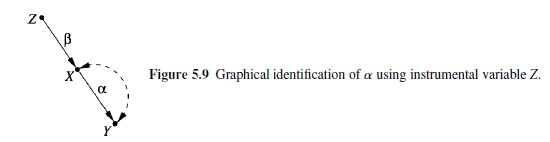
\includegraphics[width=0.8\columnwidth]{figures/instrumental-variable.jpg}  
\end{center}
\caption{Example of inference of a direct effect by evaluating a broader causal effect, and extracting the effect of interest using an instrumental variable.}
\label{Fig:instrument}
\end{figure}

Some direct effects require evaluation of a broader causal effect first, in order to extract the direct effect of interest (see Fig.~\ref{Fig:instrument}). The parameter $\alpha$ cannot be directly estimated with Theorem \ref{thm:single-door-direct-effect} because of the confounder, or its constituents (since it has none). Instead, we may apply Theorem \ref{thm:back-door-total-effect} twice like so:
\begin{align}
TE_{z,z'}(Y) = E(Y(z') - Y(z)) &= r_{YZ} = \alpha \beta \\
TE_{z,z'}(X) = E(X(z') - X(z))) &= r_{YX} = \beta \\
\alpha = E(Y|\hat{x}) &= \frac{r_{YZ}}{r_{YX}} = \frac{P(Y|\hat{z})}{P(X|\hat{z})}
\end{align}
\textbf{[I've put in the $TE_{z,z'}(Y)$ stuff myself, but this follows from Theorem \ref{thm:back-door-total-effect}, right?]}

\paragraph{To find proof:} In a linear SEM, to evaluate the partial effect of $X$ on $Y$ along a single path, take the product of all path coefficients for each endogenous edge. To evaluate the total effect for multiple branches, sum the partial effects across each branch (consisting of endogenous edges). Endogenous meaning, part of the model (i.e.\ observed).


\newpage
\bibliography{causality.bib} 

\end{document}